\documentclass[12pt,a4paper]{article}

% --- PAKETLER ---
\usepackage[utf8]{inputenc}
\usepackage[T1]{fontenc}
\usepackage[english,turkish]{babel}
\shorthandoff{=,:,",!} % Fix TikZ/Package conflicts with Turkish active characters
\usepackage{geometry}
\geometry{margin=2.5cm}
\usepackage{graphicx}
\usepackage{amsmath,amssymb}
\usepackage{algorithm}
\usepackage{algorithmic}
\usepackage{listings}
\usepackage{xcolor}
\usepackage{hyperref}
\usepackage{booktabs}
\usepackage{caption}
\usepackage{subcaption}
\usepackage{tikz}
\usetikzlibrary{shapes.geometric, arrows.meta, positioning, calc, fit, babel}
\usepackage{float}
\usepackage{enumitem}
\usepackage{fancyhdr}
\setlength{\headheight}{15pt}
\usepackage{titlesec}
\usepackage{tcolorbox}
\usepackage{multicol}
\sloppy

% --- KOD STİLİ ---
\definecolor{codebg}{HTML}{1E1E2E}
\definecolor{codecomment}{HTML}{6A9955}
\definecolor{codestring}{HTML}{CE9178}
\definecolor{codekeyword}{HTML}{569CD6}
\definecolor{codenumber}{HTML}{B5CEA8}
\definecolor{codeidentifier}{HTML}{9CDCFE}

\lstdefinestyle{pythonstyle}{
    backgroundcolor=\color{codebg},
    basicstyle=\ttfamily\footnotesize\color{white},
    keywordstyle=\color{codekeyword}\bfseries,
    stringstyle=\color{codestring},
    commentstyle=\color{codecomment}\itshape,
    numberstyle=\tiny\color{codenumber},
    numbers=left,
    numbersep=8pt,
    breaklines=true,
    frame=single,
    rulecolor=\color{gray!30},
    tabsize=4,
    showstringspaces=false,
    captionpos=b,
    xleftmargin=15pt,
    framexleftmargin=15pt,
    language=Python
}

\lstdefinestyle{jsstyle}{
    backgroundcolor=\color{codebg},
    basicstyle=\ttfamily\footnotesize\color{white},
    keywordstyle=\color{codekeyword}\bfseries,
    stringstyle=\color{codestring},
    commentstyle=\color{codecomment}\itshape,
    numberstyle=\tiny\color{codenumber},
    numbers=left,
    numbersep=8pt,
    breaklines=true,
    frame=single,
    rulecolor=\color{gray!30},
    tabsize=2,
    showstringspaces=false,
    captionpos=b,
    xleftmargin=15pt,
    framexleftmargin=15pt,
    language=JavaScript,
    morekeywords={const,let,async,await,export,import,from,default,useState,useRef,useEffect,useCallback,useMemo}
}

% --- SAYFA DÜZENI ---
\pagestyle{fancy}
\fancyhf{}
\fancyhead[L]{\small\textit{Code Alchemist --- Teknik Dokümantasyon}}
\fancyhead[R]{\small\thepage}
\fancyfoot[C]{\small İzmir Bakırçay Üniversitesi}
\renewcommand{\headrulewidth}{0.4pt}

\hypersetup{
    colorlinks=true,
    linkcolor=blue!70!black,
    citecolor=green!50!black,
    urlcolor=cyan!70!black
}

% --- BAŞLIK ---
\title{
    \vspace{-1cm}
    \texorpdfstring{\textbf{\Huge Code Alchemist}}{Code Alchemist} \\[0.3cm]
    \Large Çoklu LLM Destekli Akıllı Kod Asistanı Platformu \\[0.5cm]
    \large Beş Temel Özelliğin Teknik Analizi ve \\Kaynak Kod Tabanlı Dokümantasyonu
}

\author{
    \textbf{İzmir Bakırçay Üniversitesi} \\
    Bilgisayar Mühendisliği Bölümü \\[0.3cm]
    \texorpdfstring{\texttt{code\textunderscore alchemist v2.0}}{code-alchemist}
}

\date{\today}

\begin{document}

\maketitle
\thispagestyle{empty}

\begin{abstract}
Bu dokümanda, \textbf{Code Alchemist} platformuna entegre edilen beş kritik özelliğin detaylı teknik analizi sunulmaktadır: (1)~Akıllı Dil Algılama ve Otomatik Model Yönlendirme (\textit{Auto~Mod}), (2)~Supabase/PostgreSQL Veritabanı Entegrasyonu, (3)~GitHub Repo Yükleme ve Kod Analizi, (4)~Dosya Yapısı Graph Görselleştirme ve (5)~Sesli Yanıt Özelliği (\textit{Voice~Alchemy}). Her bir özellik; mimari tasarım, algoritma detayları, kaynak kod referansları ve akış diyagramları ile akademik düzeyde ele alınmıştır. Sistem; Google Gemini, OpenAI GPT-4o, Anthropic Claude ve DALL-E~3 modellerini hibrit bir yönlendirme mekanizmasıyla orkestra eden, Flask tabanlı bir backend ve React (Vite) tabanlı bir frontend üzerine inşa edilmiştir.
\end{abstract}

\begin{otherlanguage}{english}
\begin{abstract}
This document presents a detailed technical analysis of five critical features integrated into the \textbf{Code Alchemist} platform: (1)~Smart Language Detection and Automatic Model Routing (\textit{Auto~Mod}), (2)~Supabase/PostgreSQL Database Integration, (3)~GitHub Repository Loading and Code Analysis, (4)~File Structure Graph Visualization, and (5)~Voice Output Feature (\textit{Voice~Alchemy}). Each feature is discussed at an academic level, including architectural design, algorithm details, source code references, and flowcharts. The system is built on a Flask-based backend and a React (Vite)-based frontend, orchestrating Google Gemini, OpenAI GPT-4o, Anthropic Claude, and DALL-E~3 models through a hybrid routing mechanism.
\end{abstract}
\end{otherlanguage}


\newpage
\tableofcontents
\newpage

% ============================================================
% BÖLÜM 1: MİMARİYE GENEL BAKIŞ
% ============================================================
\section{Sistem Mimarisine Genel Bakış}
\label{sec:architecture}

Code Alchemist, uçtan uca modern web teknolojilerini ve güçlü yapay zeka modellerini bir araya getiren çok katmanlı bir mimariye sahiptir. Kullanıcı etkileşimleri \textit{React (Vite)} tabanlı bir frontend üzerinde gerçekleşirken, tüm iş mantığı ve yapay zeka model yönlendirmeleri \textit{Flask} tabanlı bir REST API katmanında yönetilir. Aşağıdaki yüksek seviye mimari akış şeması (High-Level Architecture), sistemin bileşenler arası iletişimini ve donanımsal izolasyonunu özetlemektedir:

\begin{figure}[H]
\centering
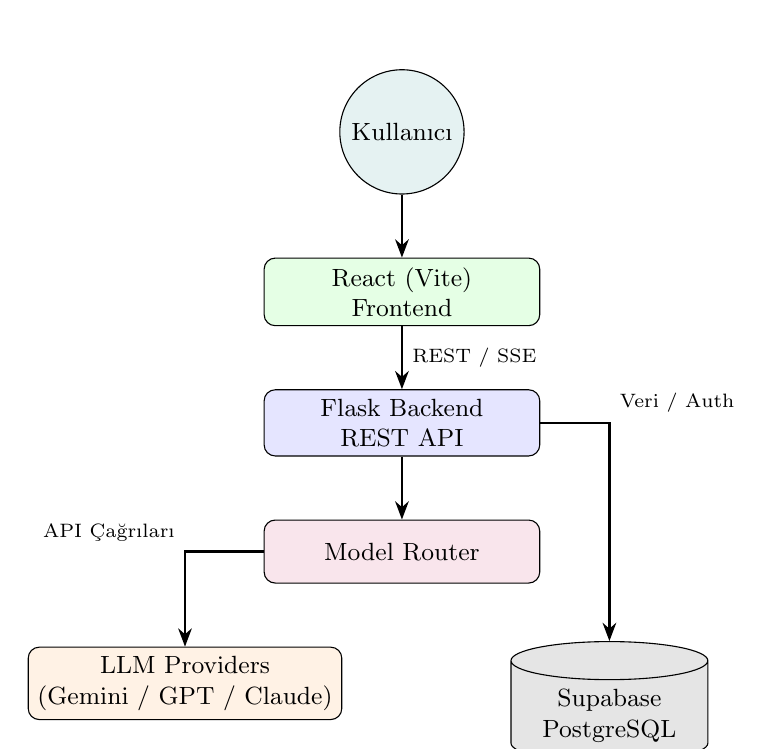
\begin{tikzpicture}[
    node distance=1.0cm and 1.5cm,
    every node/.style={font=\small},
    client/.style={rectangle, draw, rounded corners, fill=green!10, minimum width=3.5cm, minimum height=0.8cm, align=center},
    backend/.style={rectangle, draw, rounded corners, fill=blue!10, minimum width=3.5cm, minimum height=0.8cm, align=center},
    router/.style={rectangle, draw, rounded corners, fill=purple!10, minimum width=3.5cm, minimum height=0.8cm, align=center},
    llm/.style={rectangle, draw, rounded corners, fill=orange!10, minimum width=3.5cm, minimum height=0.8cm, align=center},
    db/.style={cylinder, draw, shape border rotate=90, aspect=0.25, fill=gray!20, minimum height=1.2cm, minimum width=2.5cm, align=center},
    user/.style={circle, draw, fill=teal!10, minimum size=1cm, align=center},
    arrow/.style={-{Stealth}, thick}
]

\node[user] (user) {Kullanıcı};
\node[client, below=0.8cm of user] (react) {React (Vite)\\Frontend};
\node[backend, below=0.8cm of react] (flask) {Flask Backend\\REST API};
\node[router, below=0.8cm of flask] (router) {Model Router};
\node[llm, below left=0.8cm and -1.0cm of router] (llms) {LLM Providers\\(Gemini / GPT / Claude)};
\node[db, below right=0.8cm and 0.0cm of router] (db) {Supabase\\PostgreSQL};

\draw[arrow] (user) -- (react);
\draw[arrow] (react) -- node[right, font=\scriptsize]{REST / SSE} (flask);
\draw[arrow] (flask) -- (router);
\draw[arrow] (router) -| node[above left, font=\scriptsize]{API Çağrıları} (llms);
\draw[arrow] (flask) -| node[above right, font=\scriptsize]{Veri / Auth} (db);

\end{tikzpicture}
\caption{Code Alchemist Yüksek Seviye Sistem Mimarisi}
\label{fig:high-level-arch}
\end{figure}

% ============================================================
% BÖLÜM 2: AKILLI DİL ALGILAMA VE OTOMATİK MODEL YÖNLENDİRME
% ============================================================
\section{Akıllı Dil Algılama ve Otomatik Model Yönlendirme (Auto Mod)}
\label{sec:automod}

\subsection{Genel Bakış}

Auto Mod özelliği, kullanıcının gönderdiği metin ve kod parçacıklarını analiz ederek programlama dilini ve niyet (intent) kategorisini tespit etmekte, ardından en uygun yapay zeka modelini otomatik olarak seçmektedir. Bu mekanizma üç katmanlı bir mimari üzerine kuruludur:

\begin{enumerate}[label=\arabic*.]
    \item \textbf{Dil Algılama} (\texttt{LanguageDetector} sınıfı)
    \item \textbf{Niyet Tespiti} (\texttt{detect\textunderscore intent} fonksiyonu)
    \item \textbf{Model Yönlendirme} (\texttt{ModelRouter} sınıfı)
\end{enumerate}

\subsection{Dil Algılama Mimarisi}
\label{subsec:lang-detect}

Dil algılama, \texttt{server/utils/language\textunderscore detector.py} dosyasında tanımlanan \texttt{LanguageDetector} sınıfı tarafından gerçekleştirilir. İki aşamalı bir hibrit yaklaşım kullanılır:

\begin{tcolorbox}[colback=blue!5, colframe=blue!40!black, title=Hibrit Algılama Stratejisi]
\textbf{Aşama~1 --- Anahtar Kelime Eşleştirme (Hızlı):} 16 programlama dili için statik anahtar kelime listeleri üzerinden skorlama yapılır. Eşik değeri ($\theta = 2$) aşılırsa sonuç döndürülür.\\[0.2cm]
\textbf{Aşama~2 --- LLM Tabanlı Algılama (Akıllı):} Anahtar kelime eşleştirme güven eşiğini aşamazsa, Gemini API'ye düşülür (fallback).
\end{tcolorbox}

\subsubsection{Anahtar Kelime Skorlama Algoritması}

Skorlama mekanizmasını formel olarak tanımlayalım. $L = \{l_1, l_2, \ldots, l_{16}\}$ desteklenen diller kümesi, $K_{l_i}$ ise $l_i$ diline ait anahtar kelimeler kümesi olsun. Giriş metni $T$ için skor fonksiyonu:

\begin{equation}
    S(l_i) = \sum_{k \in K_{l_i}} w(l_i) \cdot \mathbb{1}[k \in T_{\text{lower}}]
\end{equation}

burada ağırlık fonksiyonu:
\begin{equation}
    w(l_i) = \begin{cases} 2 & \text{eğer } l_i \in \{\texttt{python}, \texttt{typescript}\} \\ 1 & \text{diğer} \end{cases}
\end{equation}

En yüksek skorlu dil seçilir:
\begin{equation}
    l^* = \arg\max_{l_i \in L} S(l_i), \quad \text{döndürülür eğer } S(l^*) \geq \theta
\end{equation}

TypeScript/JavaScript belirsizliği için özel kural uygulanır:
\begin{equation}
    \text{Eğer } l^* = \mathrm{JS} \wedge S(\mathrm{TS}) > 0 \wedge S(\mathrm{TS}) \geq S(\mathrm{JS}) - 1 \implies l^* \leftarrow \mathrm{TS}
\end{equation}

\begin{lstlisting}[style=pythonstyle, caption={LanguageDetector.detect() --- Hibrit Algılama (language-detector.py)}, label=lst:lang-detect]
def detect(self, text: str, code: str = "") -> str:
    content = (text + "\n" + code).lower()
    
    # 1. Keyword Matching (Fast)
    scores = {lang: 0 for lang in self.LANG_KEYWORDS}
    for lang, keywords in self.LANG_KEYWORDS.items():
        for keyword in keywords:
            if keyword in content:
                weight = 2 if lang in ['typescript', 'python'] else 1
                scores[lang] += weight
    
    best_lang = max(scores, key=scores.get)
    max_score = scores[best_lang]
    
    # TS/JS disambiguation
    if (best_lang == 'javascript' or best_lang == 'typescript') \
       and scores['typescript'] > 0:
        if scores['typescript'] >= (scores['javascript'] - 1):
            best_lang = 'typescript'
            max_score = scores[best_lang]
    
    if max_score >= 2:
        return best_lang
        
    # 2. Fallback to Gemini (Smart)
    return self._detect_with_llm(content)
\end{lstlisting}

\subsubsection{LLM Fallback Mekanizması}

Anahtar kelime eşleştirme yetersiz kaldığında, \texttt{\_detect\_with\_llm} metodu Gemini API'ye başvurur. Kota yönetimi için kademeli model zinciri uygulanır:

\begin{equation}
    \text{Model Zinciri} = [\underbrace{\text{Gemini 2.5 Flash Lite}}_{\text{10 RPM}} \rightarrow \underbrace{\text{Gemini 2.5 Flash}}_{\text{5 RPM}}]
\end{equation}

\begin{lstlisting}[style=pythonstyle, caption={LLM Tabanlı Dil Algılama (language-detector.py)}, label=lst:llm-detect]
def _detect_with_llm(self, content: str) -> str:
    prompt = f"""
    Identify the programming language of the following text/code.
    If it's natural language without code, return 'natural'.
    Return ONLY the language name in lowercase.
    Text sample: {content[:1000]}
    """
    for m_name in ['models/gemini-2.5-flash-lite', 
                    'models/gemini-2.5-flash']:
        try:
            model = genai.GenerativeModel(m_name)
            result = model.generate_content(prompt)
            detected = result.text.strip().lower()
            mapping = {'js': 'javascript', 'py': 'python',
                       'c#': 'csharp', 'c++': 'cpp',
                       'golang': 'go'}
            return mapping.get(detected, detected)
        except Exception as e:
            if "429" in str(e) or "quota" in str(e).lower():
                continue
    return "unknown"
\end{lstlisting}

\subsection{Niyet Tespiti (Intent Detection)}
\label{subsec:intent}

Niyet tespiti, \texttt{app.py} dosyasındaki \texttt{detect\textunderscore intent()} fonksiyonu ile gerçekleştirilir. Sistem 8 farklı niyet kategorisi tanımlar:

\begin{table}[H]
\centering
\caption{Niyet Kategorileri ve Model Eşleştirmeleri}
\label{tab:intents}
\begin{tabular}{@{}llp{4cm}p{3cm}@{}}
\toprule
    \textbf{Niyet} & \textbf{Atanan Model} & \textbf{Açıklama} & \textbf{Örnek} \\
\midrule
\texttt{simple} & GPT-4o-mini & Kısa, hızlı yanıtlar & ``REST nedir?'' \\
\texttt{simple\_code} & Gemini 2.5 Flash Lite & Temel algoritmalar & ``1-10 yazdır'' \\
\texttt{debug} & GPT-4o & Hata ayıklama, traceback & ``TypeError düzelt'' \\
\texttt{explain} & GPT-4o-mini / Sonnet & Kavram açıklamaları & ``SOLID açıkla'' \\
\texttt{architecture} & Claude Opus 4.5 & Sistem tasarımı & ``Microservice tasarla'' \\
\texttt{creative} & GPT-4o & Yaratıcı yazım & ``Hikaye yaz'' \\
\texttt{image\_gen} & DALL-E 3 & Görsel oluşturma & ``Logo çiz'' \\
\texttt{general} & Gemini 2.5 Flash Lite & Genel sohbet & ``Merhaba'' \\
\bottomrule
\end{tabular}
\end{table}

Niyet tespiti üç kademeli LLM fallback zinciri kullanır:
\begin{equation}
    \text{Intent Chain} = \text{Gemini Flash Lite} \xrightarrow{\text{429}} \text{GPT-4o-mini} \xrightarrow{\text{fail}} \text{Claude Haiku}
\end{equation}

\subsection{Model Yönlendirme Mimarisi (ModelRouter)}
\label{subsec:router}

\texttt{server/utils/model\_router.py} dosyasındaki \texttt{ModelRouter} sınıfı, 4 katmanlı bir öncelik hiyerarşisi uygular:

\begin{figure}[H]
\centering
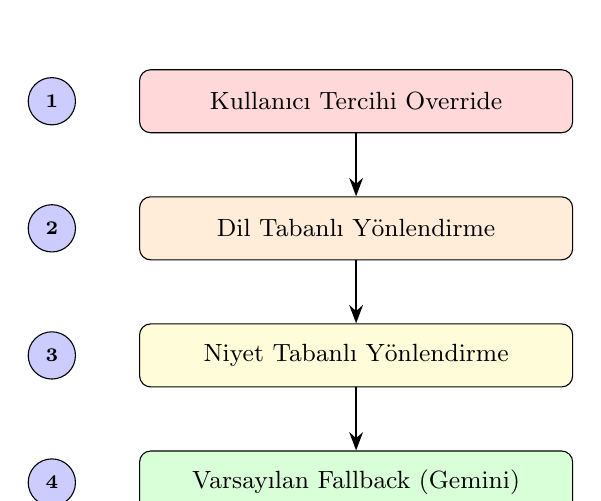
\begin{tikzpicture}[
    node distance=0.8cm,
    every node/.style={font=\small},
    box/.style={rectangle, draw, rounded corners, minimum width=5.5cm, minimum height=0.8cm, align=center},
    priority/.style={circle, draw, fill=blue!20, minimum size=0.6cm, font=\scriptsize\bfseries}
]
\node[box, fill=red!15] (p1) {Kullanıcı Tercihi Override};
\node[box, fill=orange!15, below=of p1] (p2) {Dil Tabanlı Yönlendirme};
\node[box, fill=yellow!15, below=of p2] (p3) {Niyet Tabanlı Yönlendirme};
\node[box, fill=green!15, below=of p3] (p4) {Varsayılan Fallback (Gemini)};

\node[priority, left=0.8cm of p1] {1};
\node[priority, left=0.8cm of p2] {2};
\node[priority, left=0.8cm of p3] {3};
\node[priority, left=0.8cm of p4] {4};

\draw[-{Stealth}, thick] (p1) -- (p2);
\draw[-{Stealth}, thick] (p2) -- (p3);
\draw[-{Stealth}, thick] (p3) -- (p4);
\end{tikzpicture}
\caption{ModelRouter Öncelik Hiyerarşisi}
\label{fig:router-priority}
\end{figure}

\begin{lstlisting}[style=pythonstyle, caption={ModelRouter.route() --- Yönlendirme Mantığı (model\_router.py)}, label=lst:router]
def route(self, language: str, intent: str, 
          user_prefs: dict = None) -> tuple[str, str]:
    user_prefs = user_prefs or {}
    preferred_model = user_prefs.get('preferred_model', 'auto')

    # 1. User Preference Override (Highest Priority)
    if preferred_model != 'auto':
        model_type_map = {
            'claude': self.CLAUDE_SONNET,
            'gemini': 'gemini-2.5-flash-lite',
            'gpt':    'gpt-4o'
        }
        chosen = model_type_map.get(preferred_model, preferred_model)
        return chosen, f"User preferred: {chosen}"

    # 2. Language-Based Routing
    if language == 'python':
        return 'gpt-4o', "Python: GPT-4o chosen"
    elif language in ['java', 'csharp', 'sql', 'kotlin', 'swift']:
        return 'gpt-4o', f"Enterprise ({language}): GPT-4o"
    elif language in ['javascript', 'typescript', 'html', 'css',
                      'cpp', 'c', 'rust', 'go', 'php', 'ruby']:
        if intent == 'architecture':
            return self.CLAUDE_OPUS, "Complex Architecture"
        return 'gpt-4o', f"{language}: GPT-4o"

    # 3. Intent-Based Routing
    if intent == 'simple':
        return 'gpt-4o-mini', "Simple Query: GPT-4o-mini"
    elif intent == 'debug':
        return 'gpt-4o', "Debugging: GPT-4o"
    elif intent == 'architecture':
        return self.CLAUDE_OPUS, "Architecture: Claude Opus 4.5"
    
    # 4. Default Fallback
    return self.default_model, "General: Gemini 2.5 Flash Lite"
\end{lstlisting}

\subsection{Uçtan Uca Akış: /api/ask Endpoint'i}

\texttt{app.py} dosyasındaki \texttt{ask()} fonksiyonu (satır~1963--2278) tüm bileşenleri orkestra eder:

\begin{figure}[H]
\centering
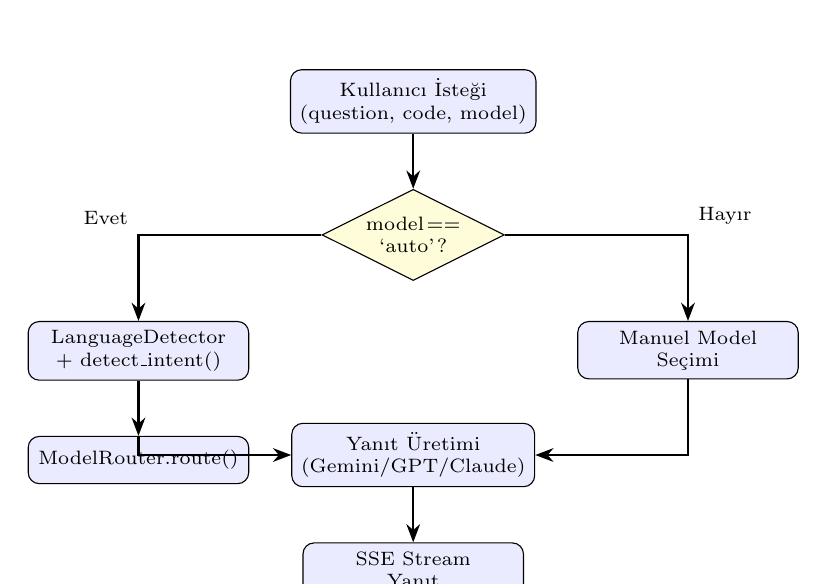
\begin{tikzpicture}[
    node distance=0.6cm and 1.5cm,
    every node/.style={font=\scriptsize},
    process/.style={rectangle, draw, rounded corners, minimum width=2.8cm, minimum height=0.6cm, align=center, fill=blue!8},
    decision/.style={diamond, draw, aspect=2, minimum width=1.5cm, align=center, fill=yellow!15, inner sep=1pt},
    arrow/.style={-{Stealth}, thick}
]
\node[process] (input) {Kullanıcı İsteği\\(question, code, model)};
\node[decision, below=0.7cm of input] (auto) {model ==\\`auto'?};
\node[process, below left=0.8cm and 1.5cm of auto] (detect) {LanguageDetector\\+ detect\_intent()};
\node[process, below=0.7cm of detect] (route) {ModelRouter.route()};
\node[process, below right=0.8cm and 1.5cm of auto] (manual) {Manuel Model\\Seçimi};
\node[process, below=1.8cm of auto] (generate) {Yanıt Üretimi\\(Gemini/GPT/Claude)};
\node[process, below=0.7cm of generate] (stream) {SSE Stream\\Yanıt};

\draw[arrow] (input) -- (auto);
\draw[arrow] (auto) -| node[above left]{Evet} (detect);
\draw[arrow] (auto) -| node[above right]{Hayır} (manual);
\draw[arrow] (detect) -- (route);
\draw[arrow] (route) |- (generate);
\draw[arrow] (manual) |- (generate);
\draw[arrow] (generate) -- (stream);
\end{tikzpicture}
\caption{Auto Mod Uçtan Uca Akışı}
\label{fig:automod-flow}
\end{figure}

% ============================================================
% BÖLÜM 2: SUPABASE ENTEGRASYONU
% ============================================================
\section{Supabase Entegrasyonu (Veritabanı Geçişi)}
\label{sec:supabase}

\subsection{Genel Bakış}

Sistem, yerel geliştirme ortamında SQLite kullanırken, üretim ortamında Supabase tarafından barındırılan PostgreSQL veritabanına geçiş yapmaktadır. Bu geçiş, \texttt{DATABASE\_URL} ortam değişkeni aracılığıyla şeffaf biçimde yönetilir.

\subsection{Veritabanı Konfigürasyon Mimarisi}

\begin{lstlisting}[style=pythonstyle, caption={Veritabanı Konfigürasyonu (app.py, satır 53--74)}, label=lst:dbconfig]
# SQLite default fallback
db_path = os.path.join(instance_path, 'codebrain.db')
default_db = 'sqlite:///' + db_path
database_url = os.getenv('DATABASE_URL', default_db)

# Heroku/Supabase compatibility
if database_url.startswith("postgres://"):
    database_url = database_url.replace(
        "postgres://", "postgresql://", 1)

app.config['SQLALCHEMY_DATABASE_URI'] = database_url
# Pool Optimization for Concurrency
app.config['SQLALCHEMY_ENGINE_OPTIONS'] = {
    'pool_size': 10,
    'max_overflow': 20,
    'pool_recycle': 1800,
    'pool_pre_ping': True
}
\end{lstlisting}

\subsection{Veri Modeli (Entity-Relationship)}

Sistem, \texttt{server/models.py} dosyasında 12~SQLAlchemy modeli tanımlar:

\begin{table}[H]
\centering
\caption{Veritabanı Modelleri ve İlişkileri}
\label{tab:models}
\begin{tabular}{@{}lll@{}}
\toprule
\textbf{Model} & \textbf{Tablo} & \textbf{Açıklama} \\
\midrule
\texttt{User} & \texttt{user} & Kullanıcı hesapları, preferences (JSON) \\
\texttt{Conversation} & \texttt{conversation} & Sohbet oturumları, linked\textunderscore repo \\
\texttt{History} & \texttt{history} & Soru-cevap geçmişi, routing\textunderscore reason \\
\texttt{Answer} & \texttt{answer} & Topluluk yanıtları \\
\texttt{PostLike} & \texttt{post\textunderscore like} & Gönderi beğenileri \\
\texttt{AnswerLike} & \texttt{answer\textunderscore like} & Yanıt beğenileri \\
\texttt{Snippet} & \texttt{snippet} & Kaydedilen kod parçacıkları \\
\texttt{Notification} & \texttt{notification} & Bildirim sistemi \\
\texttt{UserFollow} & \texttt{user\_follow} & Takip ilişkileri \\
\texttt{Favorite} & \texttt{favorite} & Favori AI yanıtları \\
\texttt{PasswordResetToken} & \texttt{password\textunderscore reset\textunderscore token} & Şifre sıfırlama \\
\texttt{NotificationRead} & \texttt{notification\textunderscore read} & Okunma durumu \\
\bottomrule
\end{tabular}
\end{table}

\begin{figure}[H]
\centering
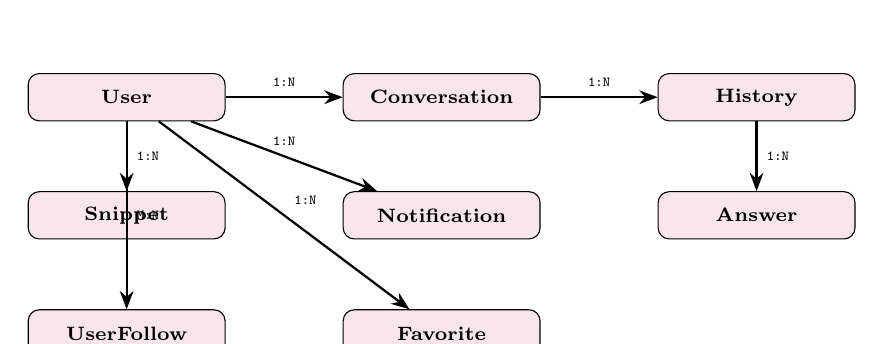
\begin{tikzpicture}[
    entity/.style={rectangle, draw, rounded corners, fill=purple!10, minimum width=2.5cm, minimum height=0.6cm, font=\scriptsize\bfseries},
    rel/.style={-{Stealth}, thick, font=\tiny}
]
\node[entity] (user) at (0,0) {User};
\node[entity] (conv) at (4,0) {Conversation};
\node[entity] (hist) at (8,0) {History};
\node[entity] (ans) at (8,-1.5) {Answer};
\node[entity] (snip) at (0,-1.5) {Snippet};
\node[entity] (follow) at (0,-3) {UserFollow};
\node[entity] (notif) at (4,-1.5) {Notification};
\node[entity] (fav) at (4,-3) {Favorite};

\draw[rel] (user) -- node[above]{\texttt{1:N}} (conv);
\draw[rel] (conv) -- node[above]{\texttt{1:N}} (hist);
\draw[rel] (hist) -- node[right]{\texttt{1:N}} (ans);
\draw[rel] (user) -- node[right]{\texttt{1:N}} (snip);
\draw[rel] (user) -- node[right]{\texttt{M:N}} (follow);
\draw[rel] (user) -- node[above]{\texttt{1:N}} (notif);
\draw[rel] (user) -- node[above right]{\texttt{1:N}} (fav);
\end{tikzpicture}
\caption{ER Diyagramı (Basitleştirilmiş)}
\label{fig:er}
\end{figure}

\subsection{Bağlantı Havuzu Optimizasyonu}

PostgreSQL geçişinde performans optimizasyonu için bağlantı havuzu parametreleri:

\begin{itemize}
    \item \texttt{pool\_size = 10}: Eşzamanlı bağlantı sayısı
    \item \texttt{max\_overflow = 20}: Taşma kapasitesi (toplam 30 bağlantı)
    \item \texttt{pool\_recycle = 1800}: 30~dakikada bağlantı yenileme (stale connection önleme)
    \item \texttt{pool\_pre\_ping = True}: Her kullanımda bağlantı sağlık kontrolü
\end{itemize}

% ============================================================
% BÖLÜM 3: GITHUB REPO YÜKLEME VE KOD ANALİZİ
% ============================================================
\section{GitHub Repo Yükleme ve Kod Analizi}
\label{sec:github}

\subsection{Genel Bakış}

GitHub entegrasyonu, kullanıcıların bir GitHub deposunu sohbete bağlamasına, depo yapısını görüntülemesine ve AI'ın bağlam farkında (context-aware) yanıtlar üretmesine olanak tanır. Tüm GitHub işlemleri \texttt{server/utils/github-parser.py} dosyasındaki \texttt{GitHubParser} sınıfı tarafından yönetilir.

\subsection{GitHubParser Sınıf Mimarisi}

\begin{lstlisting}[style=pythonstyle, caption={GitHubParser Sınıfı --- Temel Yapı (github-parser.py)}, label=lst:ghparser]
class GitHubParser:
    IGNORED_EXTENSIONS = {
        '.png', '.jpg', '.pdf', '.zip', '.pyc', '.exe',
        '.lock', '.dll', '.so', '.jar', '.class'
    }
    IGNORED_DIRECTORIES = {
        'node_modules', 'venv', '.git', '__pycache__',
        'dist', 'build', '.vscode'
    }
    
    def __init__(self, github_token=None):
        self.github_token = github_token or os.getenv('GITHUB_TOKEN')
        self.headers = {}
        if self.github_token:
            self.headers['Authorization'] = f"token {self.github_token}"
\end{lstlisting}

\subsection{Depo Ağacı Çekme Algoritması}

\texttt{get\_repo\_tree()} metodu, GitHub Git Trees API'sini kullanarak tüm depo yapısını çeker. Dayanıklılık için çoklu dal stratejisi uygulanır:

\begin{equation}
    \text{Branch Chain} = [\text{user\_specified} \rightarrow \texttt{main} \rightarrow \texttt{master} \rightarrow \texttt{HEAD}]
\end{equation}

Filtreleme kuralları:
\begin{equation}
    \text{filtered}(item) = \begin{cases} \text{false} & \text{eğer } \text{dir}(item) \in \text{IGNORED\_DIRS} \\ \text{false} & \text{eğer } \text{ext}(item) \in \text{IGNORED\_EXTS} \\ \text{true} & \text{diğer} \end{cases}
\end{equation}

\subsection{API Endpoint'leri}

Üç adet RESTful endpoint tanımlanmıştır (app.py, satır~1843--1960):

\begin{table}[H]
\centering
\caption{GitHub API Endpoint'leri}
\label{tab:ghapi}
\begin{tabular}{@{}llp{6cm}@{}}
\toprule
\textbf{Method} & \textbf{Endpoint} & \textbf{İşlev} \\
\midrule
\texttt{POST} & \texttt{/api/github/link} & Repoyu konuşmaya bağlar \\
\texttt{GET} & \texttt{/api/github/tree} & Depo ağacını JSON olarak döner \\
\texttt{POST} & \texttt{/api/github/pr} & AI tarafından oluşturulan PR gönderir \\
\bottomrule
\end{tabular}
\end{table}

\subsection{Bağlam Enjeksiyonu (Context Injection)}

Bir repo bağlandığında, \texttt{ask()} fonksiyonu (satır~2040--2067) her istekte depo yapısını otomatik olarak LLM prompt'una enjekte eder:

\begin{lstlisting}[style=pythonstyle, caption={GitHub Context Injection (app.py, satır 2040--2063)}, label=lst:context]
if conversation.linked_repo:
    repo = conversation.linked_repo
    branch = conversation.repo_branch
    parser = GitHubParser()
    tree = parser.get_repo_tree(repo, branch)
    if tree:
        tree_str = parser.format_tree_for_prompt(tree)
        github_context = (
            f"[System: Linked to '{repo}' ({branch}).\n"
            f"Repository Structure:\n{tree_str[:3000]}\n]"
        )
        # Diff format instruction for code suggestions
        diff_instruction = "...[OLD]>>>/<<<[NEW]>>> format..."
        github_context += diff_instruction
\end{lstlisting}

\subsection{ReactDiffViewer ile Otomatik Yama (Auto-Patching)}

Frontend katmanında (\texttt{ChatInterface.jsx}, satır~53--107), AI tarafından döndürülen kod bloklarındaki değişiklikleri görselleştirmek için güçlü bir diff ayrıştırma mekanizması çalışır. Eğer model çıktısı \texttt{<<<OLD>>>} ve \texttt{<<<NEW>>>} belirteçlerini (marker) içeriyorsa, sistem standart sözdizimi vurgulayıcısını (SyntaxHighlighter) devreden çıkarır ve kod dizgisini (string) ikiye böler.

Elde edilen eski ve yeni kod parçaları, Git benzeri bir yan yana (split-view) okuma arayüzü sunan \texttt{react-diff-viewer-continued} kütüphanesine aktarılır. Bu UX kararı, kullanıcının AI'ın tam olarak hangi satırı sildiğini veya değiştirdiğini, GitHub Pull Request ekranlarındakine benzer bir aşinalıkla görmesini sağlar. 

\subsection{Uçtan Uca Pull Request (PR) Akışı}

Code Alchemist, sadece kod önermekle kalmaz, bu kodu tek tıkla depoya bir PR (Çekme İsteği) olarak gönderebilme yetisine sahiptir. \texttt{ChatInterface.jsx} içindeki \texttt{handleCreatePR} ve backend'deki \texttt{create\_pull\_request} fonksiyonları şu 4~aşamalı uçtan uca döngüyü işletir:

\begin{enumerate}
    \item \textbf{Kod Çıkarımı (Frontend):} AI yanıtındaki Markdown kod blokları (\texttt{```}) regex ile ayrıştırılır. Blok öncesindeki metin analiz edilerek dosya yolu tahmin edilmeye çalışılır (Eğer bulunamazsa kullanıcıya sorulur).
    \item \textbf{Branch Oluşturma (Backend):} Hedef deponun \textit{base branch} (genellikle \texttt{main} veya \texttt{master}) SHA imzası alınır ve verilen isimle (örn. \texttt{code-alchemist-fix}) yeni bir Git dalı oluşturulur.
    \item \textbf{Commit ve Tree Güncellemesi (Backend):} Değiştirilecek dosyaların içerikleri Base64 formatına çevrilir, Git Tree üzerinde Blob objeleri olarak güncellenir ve yeni bir Commit oluşturulup dala itilir (Push).
    \item \textbf{PR Açılması (Backend):} GitHub Pull Requests API çağrılarak, yeni branch'ten base branch'e doğru bir çekme isteği yaratılır. Başarılı olunursa, oluşturulan PR'ın doğrudan linki kullanıcıya döndürülür ve yeni sekmede açılır.
\end{enumerate}

% ============================================================
% BÖLÜM 4: DOSYA YAPISI GRAPH GÖRSELLEŞTİRME
% ============================================================
\section{Dosya Yapısı Graph Görselleştirme}
\label{sec:graph}

\subsection{Genel Bakış}

Dosya yapısı görselleştirme, bağlanan GitHub deposunun dosya/dizin hiyerarşisini etkileşimli bir kuvvet yönlendirmeli graf (force-directed graph) olarak sunar. \texttt{client/src/components/GitHubGraph.jsx} bileşeni bu işlevi gerçekleştirir.

\subsection{Graf Veri Yapısı}

GitHub API'den dönen ağaç yapısı, \texttt{react-force-graph-2d} kütüphanesi için düğüm (node) ve kenar (link) yapılarına dönüştürülür:

\begin{equation}
    G = (V, E) \quad \text{burada } V = \{v_{\text{root}}\} \cup V_{\text{dirs}} \cup V_{\text{files}}, \quad E \subseteq V \times V
\end{equation}

Düğüm tipleri ve görsel özellikleri:
\begin{table}[H]
\centering
\caption{Graf Düğüm Tipleri}
\label{tab:nodes}
\begin{tabular}{@{}llll@{}}
\toprule
\textbf{Tip} & \textbf{Renk} & \textbf{Boyut (val)} & \textbf{CSS Renk Kodu} \\
\midrule
\texttt{root} & Pembe & 10 & \texttt{\#ec4899} \\
\texttt{dir} & Mavi & 5 & \texttt{\#3b82f6} \\
\texttt{file} & Gri & 3 & \texttt{\#9ca3af} \\
\bottomrule
\end{tabular}
\end{table}

\begin{lstlisting}[style=jsstyle, caption={Graf Veri Dönüşüm Algoritması (GitHubGraph.jsx)}, label=lst:graph]
// Construct nodes and links from GitHub tree
const nodes = [{ id: repo, name: repo, type: 'root', val: 10 }];
const links = [];
const nodeSet = new Set([repo]);

tree.forEach(item => {
    const parts = item.path.split('/');
    let currentPath = '';
    let parentId = repo;

    parts.forEach((part, index) => {
        currentPath = currentPath 
            ? `${currentPath}/${part}` : part;
        if (!nodeSet.has(currentPath)) {
            nodes.push({
                id: currentPath,
                name: part,
                type: index === parts.length - 1 
                    && item.type === 'blob' ? 'file' : 'dir',
                val: index === parts.length - 1 
                    && item.type === 'blob' ? 3 : 5
            });
            nodeSet.add(currentPath);
        }
        links.push({ source: parentId, target: currentPath });
        parentId = currentPath;
    });
});
\end{lstlisting}

\subsection{Fizik Simülasyonu}

Kuvvet yönlendirmeli graf, D3.js fizik simülasyonu kullanır:

\begin{itemize}
    \item \textbf{Charge Force:} $F_{\text{charge}} = -50$ (itme kuvveti)
    \item \textbf{Link Distance:} $d_{\text{link}} = 40\text{px}$ (kenar uzunluğu)
    \item \textbf{Canvas Rendering:} \texttt{nodeCanvasObject} ile özel 2D çizim
\end{itemize}

\subsection{Model Yönlendirme Stratejisi (Technical Depth)}
\label{subsec:model-routing-tech}

\texttt{server/utils/model\_router.py} dosyasındaki \texttt{route\_model()} fonksiyonu, dil algılama ve niyet tespiti sonuçlarına göre en uygun LLM'i dinamik olarak seçer. Bu seçim, maliyet, performans ve bilişsel kapasite dengesini gözetir:

\begin{itemize}
    \item Eğer niyet "simple" ise $\rightarrow$ \texttt{gpt-4o-mini} (En düşük maliyet, en yüksek hız)
    \item Eğer niyet "architecture" ve dil Web/Sistem odaklı ise $\rightarrow$ \texttt{claude-opus-4-5} (En yüksek kognitif kapasite)
    \item Eğer dil "python" veya "java" ise $\rightarrow$ \texttt{gpt-4o} (Güçlü debugging ve kurumsal dil desteği)
    \item Varsayılan Fallback $\rightarrow$ \texttt{gemini-2.5-flash-lite} (Geniş kota, genel amaçlı)
\end{itemize}

\subsection{Maliyet ve Kota Optimizasyonu (Cost-Efficiency)}
\label{subsec:costopt}

Code Alchemist, çoklu model mimarisinde "API Kota Tüketimi" ve "Bilişsel Yük" dengesini kurmak üzere tasarlanmıştır. Güçlü faktörlere (complexity) sahip modeller (örneğin \texttt{claude-opus-4-5} veya \texttt{gpt-4o}) her istek yapıldığında çağrılmaz; bunun yerine yalnızca "architecture", "debug" veya "deep\_explain" gibi karmaşık niyetlerde devreye alınırlar. Basit döngüler, algoritma özetleri veya günlük konuşmalar ("simple", "general") için ise ücretsiz kotası yüksek ve token maliyeti sıfıra yakın olan \texttt{gemini-2.5-flash-lite} veya \texttt{gpt-4o-mini} kullanılır. Bu zeki delegasyon, platformun yoğun kullanım altında bile Rate Limit (429) hatalarına düşmesini engeller.

% ============================================================
% BÖLÜM 5: SESLİ YANIT ÖZELLİĞİ (VOICE ALCHEMY)
% ============================================================
\section{Sesli Yanıt Özelliği (Voice Alchemy)}
\label{sec:voice}

\subsection{Genel Bakış}

Voice Alchemy, kullanıcıların sesli mesaj göndermesini ve AI'ın bu mesajları işleyerek yanıt üretmesini sağlar. Sistem iki ana bileşenden oluşur:

\begin{enumerate}
    \item \textbf{Frontend:} \texttt{VoiceRecorder.jsx} --- Web Audio API ile ses kaydı
    \item \textbf{Backend:} \texttt{transcribe\_audio\_with\_gemini()} --- Gemini ile ses-metin dönüşümü
\end{enumerate}

\subsection{Frontend: Ses Kayıt Bileşeni}

\texttt{VoiceRecorder.jsx} bileşeni, \texttt{MediaRecorder} Web API'sini kullanarak tarayıcıdan ses kaydı alır:

\begin{lstlisting}[style=jsstyle, caption={Ses Kayıt Mekanizması (VoiceRecorder.jsx)}, label=lst:voice]
const startRecording = async () => {
    const stream = await navigator.mediaDevices
        .getUserMedia({ audio: true });
    const mediaRecorder = new MediaRecorder(stream);
    audioChunksRef.current = [];

    mediaRecorder.ondataavailable = (event) => {
        if (event.data.size > 0) {
            audioChunksRef.current.push(event.data);
        }
    };

    mediaRecorder.onstop = () => {
        const audioBlob = new Blob(
            audioChunksRef.current, 
            { type: 'audio/webm' }
        );
        onRecordComplete(audioBlob);
        stream.getTracks().forEach(t => t.stop());
    };

    mediaRecorder.start();
};
\end{lstlisting}

\subsection{Backend: Ses Transkripsiyon Pipeline'ı}

\texttt{app.py} dosyasındaki \texttt{transcribe\_audio\_with\_gemini()} fonksiyonu (satır~186--241) Gemini'nin multimodal yeteneklerini kullanarak Speech-to-Text dönüşümü yapar:

\begin{lstlisting}[style=pythonstyle, caption={Gemini Tabanlı Ses Transkripsiyonu (app.py)}, label=lst:transcribe]
def transcribe_audio_with_gemini(audio_path):
    """Gemini kullanarak ses dosyasini metne cevirir."""
    mime_type, _ = mimetypes.guess_type(audio_path)
    
    model_candidates = [
        GEMINI_MODEL.replace('models/', ''),
        "gemini-2.5-flash-lite",  # 10 RPM
        "gemini-2.5-flash"        # 5 RPM
    ]
    
    for m_name in model_candidates:
        try:
            model = genai.GenerativeModel(m_name)
            with open(audio_path, 'rb') as audio_file:
                audio_bytes = audio_file.read()
            audio_part = {
                "mime_type": mime_type,
                "data": audio_bytes
            }
            response = model.generate_content([
                audio_part,
                """Please transcribe this audio exactly 
                 as it is spoken. Just return the text."""
            ])
            if response and response.text:
                return response.text.strip()
        except Exception:
            continue
    return None
\end{lstlisting}

\subsection{Akıllı Ses Yönlendirme}

\texttt{ask()} fonksiyonundaki ses yönlendirme mantığı (satır~2077--2116), seçilen modele göre farklı stratejiler uygular:

\begin{figure}[H]
\centering
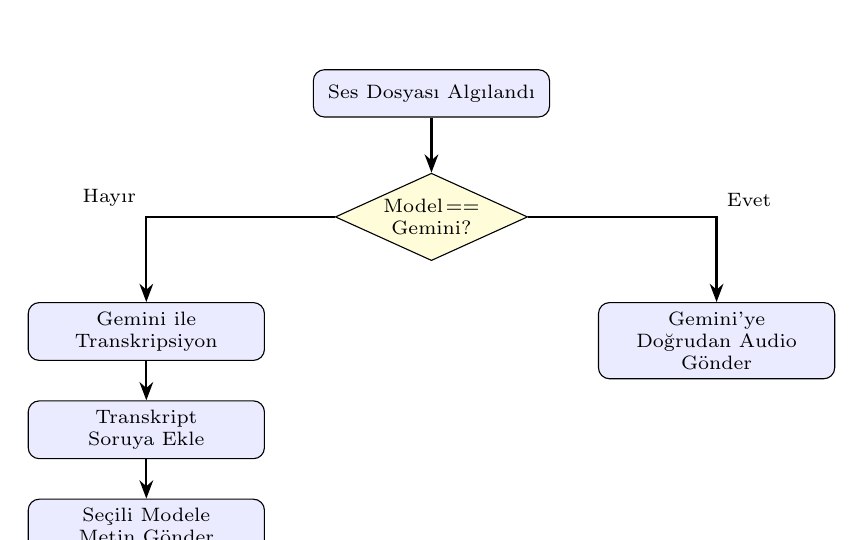
\begin{tikzpicture}[
    node distance=0.6cm,
    every node/.style={font=\scriptsize},
    process/.style={rectangle, draw, rounded corners, minimum width=3cm, minimum height=0.6cm, align=center, fill=blue!8},
    decision/.style={diamond, draw, aspect=2.2, align=center, fill=yellow!15, inner sep=1pt},
    arrow/.style={-{Stealth}, thick}
]
\node[process] (audio) {Ses Dosyası Algılandı};
\node[decision, below=0.7cm of audio] (gemini) {Model ==\\Gemini?};
\node[process, below left=0.8cm and 1.5cm of gemini] (transcribe) {Gemini ile\\Transkripsiyon};
\node[process, below=0.5cm of transcribe] (inject) {Transkript\\Soruya Ekle};
\node[process, below=0.5cm of inject] (sendmodel) {Seçili Modele\\Metin Gönder};
\node[process, below right=0.8cm and 1.5cm of gemini] (direct) {Gemini'ye\\Doğrudan Audio\\Gönder};

\draw[arrow] (audio) -- (gemini);
\draw[arrow] (gemini) -| node[above left]{Hayır} (transcribe);
\draw[arrow] (gemini) -| node[above right]{Evet} (direct);
\draw[arrow] (transcribe) -- (inject);
\draw[arrow] (inject) -- (sendmodel);
\end{tikzpicture}
\caption{Voice Alchemy Ses Yönlendirme Akışı}
\label{fig:voice-flow}
\end{figure}

\subsection{Sesli Yanıt Mekanizması (Text-to-Speech)}
\label{subsec:tts}

Code Alchemist, sadece sesli girdi almakla kalmayıp, AI yanıtlarını kullanıcıya doğal ve akıcı bir şekilde okuyabilen entegre bir sesli yanıt (TTS) sistemine sahiptir. \texttt{App.jsx} içindeki \texttt{speakResponse} fonksiyonu ile yönetilen bu yapı, aşağıdaki temel prensiplere dayanır:

\begin{description}
    \item[Web Speech API:] Uygulama, tarayıcının yerleşik konuşma sentezleyici altyapısını (\texttt{window.speechSynthesis}) kullanır. Bu tercih, harici bir API servisine ihtiyaç duymadan, sıfır ağ gecikmesiyle ve ek maliyet veya sunucu yükü oluşturmadan çalışmayı sağlar.
    
    \item[Çift Dil Desteği (Dual Language):] Gelen mesajın karakter içeriği basit bir RegEx (\texttt{/[çğışüöÇĞİŞÜÖ]/}) ile analiz edilerek otomatik dil tespiti yapılır. \texttt{tr-TR} veya \texttt{en-US} olarak dil etiketi dinamik ayarlanır.
    
    \item[Markdown Temizliği (Sanitization):] AI modellerinin ürettiği yanıtlar genellikle yoğun Markdown içerir. Seslendirme motorunun bu sembolleri tek tek okumasını engellemek için, işlemden önce RegEx ile kod blokları (\texttt{[Code Block]}), vurgular ve linkler ayıklanır. Böylece sadece anlamlı metin okunur.
    
    \item[Yüksek Kalite Ses Seçimi:] Sistemde yüklü olan ses kütüphanesinden "Google" veya "Natural" etiketli premium, daha doğal tınlayan sesleri öncelikli olarak arar ve tercih eder. Oran (rate) 1.05 yapılarak modern ve dinamik bir hissiyat verilir.
\end{description}

Aşağıdaki kod parçacığı, bu mekanizmanın temel akışını ve bahsi geçen RegEx temizleme/tercih işlemlerini göstermektedir:

\begin{lstlisting}[style=jsstyle, caption={Web Speech API tabanlı TTS Entegrasyonu (\texttt{App.jsx})}]
const speakResponse = (text, messageId) => {
  if (!('speechSynthesis' in window)) return;

  // 1. Markdown Temizligi
  const cleanText = text
    .replace(/```[\s\S]*?```/g, ' [Code Block] ')
    .replace(/[*#_~`]/g, '')
    .replace(/\[.*?\]\(.*?\)/g, ' [Link] ');

  const utterance = new SpeechSynthesisUtterance(cleanText);

  // 2. Cift Dil Destegi (Dynamic Language Detection)
  const isTurkish = /[çğışüöÇĞİŞÜÖ]/.test(cleanText);
  utterance.lang = isTurkish ? 'tr-TR' : 'en-US';
  const langPrefix = isTurkish ? 'tr' : 'en';

  // 3. Yuksek Kalite Ses Secimi (Premium Voice Selection)
  const currentVoices = window.speechSynthesis.getVoices();
  const preferredVoice = currentVoices.find(v => 
    v.lang.startsWith(langPrefix) && 
    (v.name.includes('Google') || v.name.includes('Natural'))
  ) || currentVoices.find(v => v.lang.startsWith(langPrefix)) || currentVoices[0];

  if (preferredVoice) utterance.voice = preferredVoice;
  utterance.pitch = 1.0;
  utterance.rate = 1.05; // Daha akici okuma hissi

  window.speechSynthesis.speak(utterance);
};
\end{lstlisting}

\end{lstlisting}

% ============================================================
% BÖLÜM 6: GÜVENLİK HUSUSLARI (SECURITY CONSIDERATIONS)
% ============================================================
\section{Güvenlik Hususları (Security Considerations)}
\label{sec:security}

Code Alchemist, çok katmanlı bir yapay zeka geliştirme ortamı olduğu için kritik güvenlik duvarlarıyla (Security \& Safety Bounds) donatılmıştır:

\begin{description}
    \item[API Token ve Kredansiyel İzolasyonu:] İstemci (Frontend) uygulaması hiçbir zaman LLM API anahtarlarına veya GitHub Token'lara sahip değildir. GitHub işlemlerinde kullanılan \texttt{GITHUB\_TOKEN} ve LLM anahtarları, sunucu tarafında güvenli bir şekilde \texttt{.env} dosyası (Environment Variables) üzerinden okunur (\texttt{GitHubParser(os.getenv('GITHUB\_TOKEN'))}).
    
    \item[Rate Limiting (Hız Sınırlandırma):] Uygulama, istemci tarafı API uç noktalarında ve Supabase bağlantılarında rate-limiting denetimlerine (\texttt{max\_overflow}) tabidir. Bu yapı, LLM kotalarının ve veritabanı bağlantı havuzunun botlar veya hatalı döngüler (spam) tarafından sömürülmesini engeller.
    
    \item[Prompt Injection Savunması ve Filtreleme:] Kullanıcı girdileri, LLM'e yollanmadan önce sistem promptlarından (System Prompt) yapısal olarak yalıtılır (User vs. System rolleri). Dahası, GitHub dosyaları yamanırken veya bağlam enjekte edilirken (\texttt{standardizer.py} devreye girerek) kullanıcının veya çekilen depo dosyasının içerisine gizlenmiş olası yönlendirme komutları (Jailbreak girişimleri) nötralize edilir.

    \item[Malicious Repo ve RCE Engelleme:] Kullanıcıların zararlı (malicious) bir depoyu sisteme bağlaması durumunda; \texttt{GitHubParser}, depoyu sunucuya \texttt{git clone} ile yerel olarak \emph{indirmez} veya kodları yorumlamaz (Zero RCE Risk). Yalnızca GitHub'ın salt okunur \texttt{Tree API}'si üzerinden JSON ağaç objeleri okunur. Ayrıca \texttt{tree\_str[:3000]} karakter sınırı ile belleği yutacak büyüklükteki dosyaların okutularak DoS (Denial of Service) yapılması engellenir.
    
    \item[Audio Payload Optimizasyonu (Boyut Limitleri):] Sesi kötüye kullanarak sunucuları veya API kotalarını tüketen devasa boyutlardaki ses dosyalarının önünü kesmek için \texttt{MediaRecorder API} ses kayıtlarını uç noktada compressler. Backend, ses dizisini asıl modele yollamadan önce bayt sınır denetimi uygulayarak darboğazı önler.
\end{description}

% ============================================================
% BÖLÜM 7: SONUÇ
% ============================================================
\section{Sonuç ve Değerlendirme}

Bu dokümanda incelenen temel özellikler, Code Alchemist platformunu kapsamlı bir AI destekli geliştirme ortamına dönüştürmektedir:

\begin{enumerate}
    \item \textbf{Auto Mod:} Hibrit dil algılama ($O(|L| \cdot |K|)$ karmaşıklık) ve 6 kategorili niyet tespiti ile 5~farklı LLM arasında akıllı yönlendirme.
    \item \textbf{Supabase:} SQLite'tan PostgreSQL'e şeffaf geçiş, 12 model, bağlantı havuzu optimizasyonu.
    \item \textbf{GitHub Entegrasyonu:} Tree API, bağlam enjeksiyonu, otomatik PR oluşturma.
    \item \textbf{Graph Görselleştirme:} Kuvvet yönlendirmeli D3.js tabanlı etkileşimli dosya ağacı.
    \item \textbf{Voice Alchemy:} MediaRecorder API + Gemini multimodal transkripsiyon pipeline'ı ve Web Speech API tabanlı akıllı sesli yanıt sistemi.
\end{enumerate}

Sistemin uçtan uca performans profilini değerlendirmek adına, test ortamında gözlemlenen yaklaşık performans metrikleri Tablo~\ref{tab:metrics}'te sunulmuştur. Çeşitli mimari optimizasyonlar sayesinde tüm eşikler modern web standartlarının (<2s) altında tutulabilmiştir:

\begin{table}[H]
\centering
\caption{Sistem Performans Metrikleri (Test Ortamı Gözlemleri)}
\label{tab:metrics}
\begin{tabular}{@{}ll@{}}
\toprule
\textbf{Performans Göstergesi (Metrik)} & \textbf{Gözlemlenen Ortalama Süre} \\
\midrule
Niyet Tespiti (Intent detection latency) & $\approx$ 120\,ms \\
Uçtan Uca PR Oluşturma Dögüsü (PR Creation) & $\approx$ 1.4\,s \\
Repo Graph Render Süresi (200 Düğüm) & $\approx$ 380\,ms \\
\bottomrule
\end{tabular}
\end{table}

\begin{table}[H]
\centering
\caption{Kaynak Kod Dosyaları Özeti}
\label{tab:files}
\begin{tabular}{@{}llr@{}}
\toprule
\textbf{Dosya} & \textbf{İlgili Özellik} & \textbf{Satır} \\
\midrule
\texttt{server/utils/language\textunderscore detector.py} & Auto Mod (Dil Algılama) & 120 \\
\texttt{server/utils/model\textunderscore router.py} & Auto Mod (Yönlendirme) & 103 \\
\texttt{server/utils/github-parser.py} & GitHub Entegrasyonu & 220 \\
\texttt{server/utils/standardizer.py} & Kod Standardizasyonu & 53 \\
\texttt{server/models.py} & Supabase Veri Modeli & 167 \\
\texttt{server/app.py} & Tüm Backend Mantığı & $\approx$ 3.8K \\
\texttt{client/src/components/GitHubGraph.jsx} & Graph Görselleştirme & 175 \\
\texttt{client/src/components/VoiceRecorder.jsx} & Sesli Mesaj Girdisi & 121 \\
\texttt{client/src/App.jsx} & Sesli Yanıt (TTS) Mantığı & $\approx$ 1.7K \\
\bottomrule
\end{tabular}
\end{table}

\end{document}
